This section describes methods used to estimate backgrounds from Standard Model processes in the search for $h \rightarrow aa \rightarrow bb\tau\tau$. The background contributions directly taken from MC are described in Sections \ref{section:background-estimation:z-plus-jets} to \ref{section:background-estimation:SM-higgs}. Section \ref{section:ch-7-jet-faking-tauh-background} describes the data-driven method for estimating backgrounds from jets faking hadronic tau decays (jet $\rightarrow \tau_{h}$), which is used in the $\mu\tau_{h}$ and $e\tau_{h}$ channels. Section \ref{section:ch-7-QCD-multijet-background} describes the data-driven method for estimating background from quantum chromodynamic (QCD) processes in the $e\mu$ channel.

\section{Z+jets}
\label{section:background-estimation:z-plus-jets}
A major source of background for $\tau\tau$ analyses is the Drell-Yan (DY) process (Z+jets). The Z boson decays to $\tau\tau/ \mu\mu/ ee$ with equal probability of 3.4\% each, with the dominant decay modes being to hadrons (around 70\%) and neutrinos (invisible) (20\%)~\cite{workman_review_2022}. 

The Drell-Yan contribution with genuine taus, Z $\rightarrow \tau\tau$, is estimated using embedded samples, described in Section \ref{section:embedded-samples}. To avoid double-counting between embedded and MC samples, in all MC samples, events with legs that originated from genuine $\tau$ are discarded.

The other decays of the Z, Z $\rightarrow ee$ and Z $\rightarrow \mu\mu$, are estimated from MC simulation, and are hereafter referred to as simply the Drell-Yan background. These MC samples are generated to leading order (LO) with different numbers of jets (jet multiplicity) in the matrix element: Z+1 jet, Z+2 jets, Z+3 jets, Z+4 jets, and inclusive Z+jets. The cross-sections of the samples with $\geq 1$ jets are normalized to next-to-NLO (NNLO) in QCD. For the inclusive Drell-Yan sample, two samples are used with different thresholds for the di-lepton invariant mass ($m_{\ell}$) at the generator level: one with $m_{\ell\ell} > 50$ GeV and the other with $10 < m_{\ell\ell} < 50$. 

\section{W+jets}

The dominant W boson decay modes are to hadrons (67.4\%), $e + \nu_e$ (10.7\%), $\mu + \nu_\mu$ (10.6\%), and $\tau + \nu_\tau$ (11.4\%)~\cite{workman_review_2022}.
The W+jets background is estimated from MC simulation. Similarly to the Z+jets, the W+jets samples are generated with different jet multiplicities in the matrix element. LO samples are used for greater statistics and are normalized to NNLO cross-sections. 

\section{\texorpdfstring{$t\bar{t}$}{ttbar} + jets}
In hadron collisions, top quarks are produced singly with the weak interaction, or in pairs via the strong interaction, with interference between these leading-order processes possible in higher orders of the perturbation theory. 
The top quark is the heaviest fermion in the Standard Model and has a short lifetime ($\sim 10^{-25}$ s), decaying without hadronization into a bottom quark and a W boson~\cite{workman_review_2022}, with the decay modes of the W boson as listed in the previous section. With two top quarks, the final states of the two resulting W bosons can be described as fully leptonic, semileptonic, and fully hadronic. These three final states are modeled separately with MC simulation in 2018 and 2017, while for 2016 the sample used is inclusive.

\section{Single top}
% https://cms.cern/news/measurement-t-channel-single-top-quark-production-rates-pp-collisions-7-tev
There are three main production modes of the single top in $pp$ collisions~\cite{CMS-CR-2018-185}: the exchange of a virtual W boson ($t$ channel), the production and decay of a virtual W boson ($s$ channel), and the associated production of a top quark and W boson ($tW$, or W-associated) channel. As the $s$ channel process is rare and only 3\% of the total production, the dominant production mode of the $t-channel$ and the $tW$ production are considered and modeled with MC. 

\section{Diboson}

In $pp$ collisions, the production of dibosons (pairs of electroweak gauge bosons, i.e. WW, WZ, and ZZ) is dominated by quark-antiquark annihilation, with a small contribution from gluon-gluon interactions~\cite{CMS-SMP-20-012}. MC is used to model the pair production and decays of VV to $2\ell 2\nu$, WZ to $2q 2\ell$ and $3 \ell \nu$, and ZZ to $4\ell$ and $2q 2\ell$ ($q$ being quarks and $\ell$ being leptons).

\section{Standard Model Higgs}
\label{section:background-estimation:SM-higgs}
MC is used to simulate backgrounds from major production modes of the Standard Model 125\GeV Higgs boson: gluon-gluon fusion (ggH), vector boson fusion (VBF), associated production with a W or Z (WH, ZH), and associated production with a top pair (ttH) (see Fig. \ref{fig:higgs-boson-production-modes} for leading-order diagrams). For these production modes, samples with the Higgs decaying to $\tau\tau$ or to $WW$ are used. Samples made with higher-order diagrams for WH and ZH that include the production of a jet, with the Higgs decaying to WW, are also used.

\begin{figure}[ht]
    \centering
    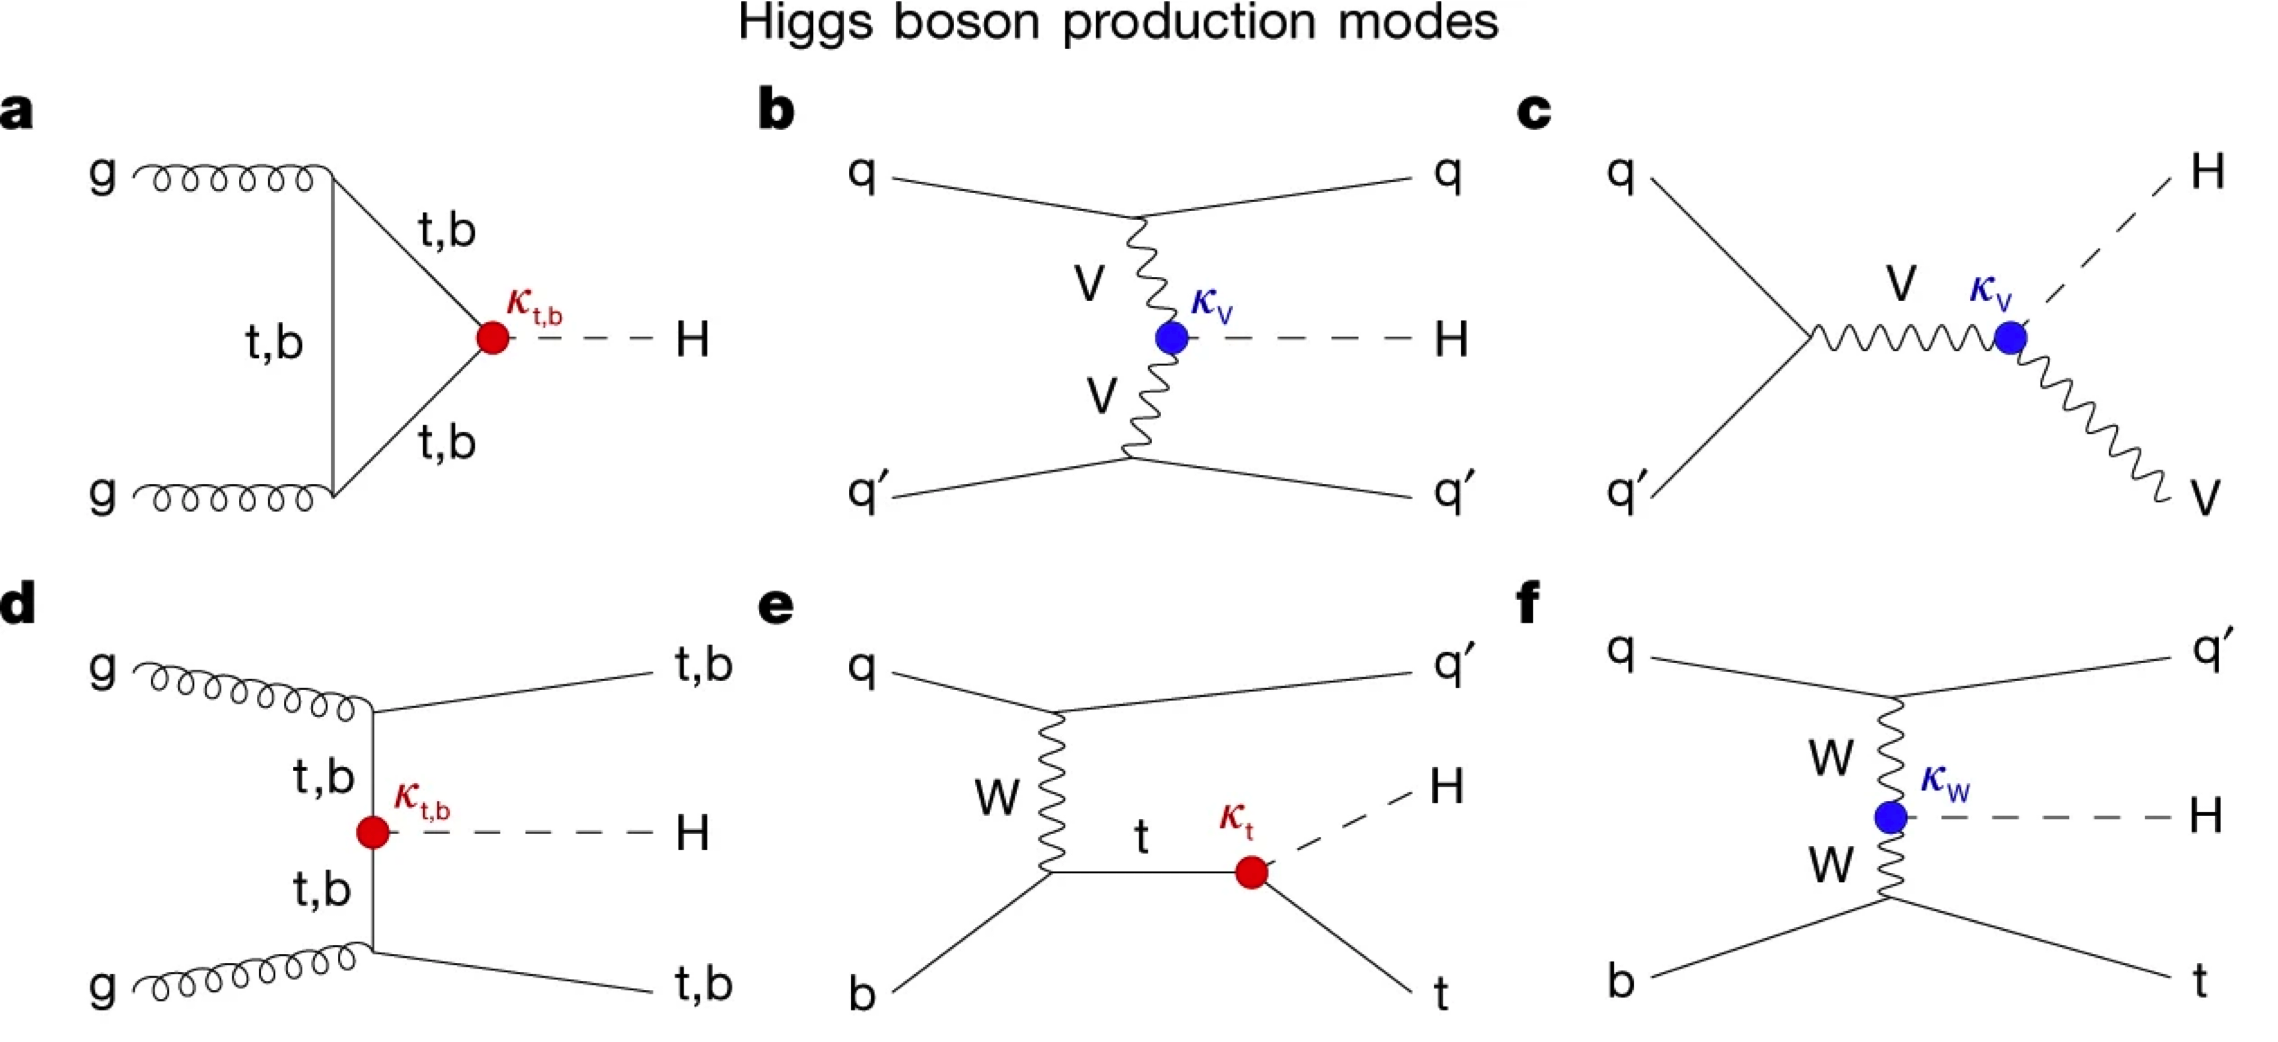
\includegraphics[width=15cm]{figures/ch-7-background-estimation/higgs-boson-production-modes.png}
    \caption[Leading-order Feynman diagrams of Higgs production.]{Leading-order Feynman diagrams of Higgs production from~\cite{CMS-HIG-22-001}, in ggH (\textit{a}) and vector boson fusion (VBF; \textit{b}), associated production with a W or Z (V) boson (VH; \textit{c}), associated production with a top or bottom quark pair (ttH or bbH); \textit{d}, and associated production with a single top quark (tH; \textit{e, f}).} 

     \label{fig:higgs-boson-production-modes}
\end{figure}

\section{Jet faking \texorpdfstring{$\tau_{h}$}{tauh}}
\label{section:ch-7-jet-faking-tauh-background}
Events with a jet mis-reconstructed as the hadronic tau leg $\tau_{h}$ are a major source of background in the $\mu\tau_{h}$ and $e\tau_{h}$ channels. The main processes contributing to jet $\rightarrow \tau_{h}$ events are QCD multijet, W+jets, and $t\bar{t}$ production. These events are estimated using a data-driven method adapted from past analyses~\cite{CMS-HIG-19-010}~\cite{CMS-HIG-17-024}. This background includes contributions from W+jets, QCD multijets, and $t\bar{t}$+jets. To estimate this background, a sideband region is constructed, where events are required to pass all baseline $\mu\tau_{h}/ e\tau_{h}$ selection criteria, but fail the $\tau_{h}$ isolation criteria. The events in this sideband region are reweighed with a factor $f/(1-f)$, where $f$ is the probability for a jet to be misidentified as a $\tau_{h}$. The jet $\rightarrow \tau_{h}$ background is the anti-isolated, reweighed MC and embedded events subtracted from the anti-isolated, reweighted data events.

The fake factor is measured in $Z \rightarrow \mu\mu$+jets events in data in the $\mu\mu\tau_{h}$ final state, as any reconstructed $\tau_{h}$ in these events must originate from a jet. The two muons are required to be isolated $(<0.15)$, have opposite electric charges, and have an invariant mass between 76 and 106 GeV (close to the Z mass). These events are selected with a double muon trigger, with the leading muon having offline $p_T > 20$ GeV and the subleading muon $p_{T} > 10$ GeV. Simulated diboson (ZZ and WZ) events are subtracted to avoid contamination from events with real $\tau_{h}$. The denominator of the fake rate corresponds to fake taus passing the VVVLoose working point of the discriminator vs. jets, while the numerator corresponds to those passing the Medium working point, i.e. $f = N_{\text{jet passing tight}}/ N_{\text{jet passing loose}}$.

$f$ is measured as a function of the $\tau_{h}$ transverse momentum and is 8\% - 10\% in each of the data-taking years. $f$ is derived separately for the $\mu\tau_{h}$ and $e\tau_{h}$ channels because the channels use different anti-lepton identification working points.

\section{QCD multijet background}
\label{section:ch-7-QCD-multijet-background}
In the $e\mu$ channel, the rate of events with jets faking electrons or muons originating from QCD multijet processes, is estimated from data events with the same baseline selection as in the signal region, except with same-signed (SS) charged $e+\mu$, ensuring orthogonality with the signal region which requires opposite-sign (OS) $e\mu$ pairs. All same-sign MC events (both events with real and fake $e+\mu$) are subtracted from same-sign data events to remove contamination from other backgrounds. i.e. QCD$_{\text{SS}}$ = Data$_{\text{SS}}$ - MC$_{\text{SS}}$.

Three scale factors are applied to the QCD$_{\text{SS}}$ events to compute the QCD multijet background~\cite{CMS-HIG-17-024}~\cite{CMS-HIG-22-007}:
\begin{itemize}
    \item \textit{OS-to-SS scale factor}: This scales the SS QCD to the OS region, and is measured from an orthogonal region with an isolated electron and an anti-isolated muon. Only the muon is chosen to be anti-isolated because this scale factor was observed to depend more strongly on electron isolation than on muon isolation. This scale factor is treated as a function of the $\Delta R$ separation of the trajectories of the electron and muon, and is measured separately for events with 0 jets, 1, jet, and greater than 1 jet.
    \item \textit{2D closure correction for the lepton $p_{T}$}: This factor accounts for subleading dependencies of the first scale factor on the $p_{T}$ of the two leptons. A 2D weight is derived in a similar fashion, as a ratio of QCD$_{OS}$ events to QCD$_{\text{SS}}$ events, but parameterized by both electron and muon $p_{T}$, where the SS events have the previous scale factor applied.
    \item \textit{Isolation correction for the muon}: The third and final factor is an isolation correction, which is a bias correction to account for the fact that the fake factor was determined for less-isolated muons. This factor is obtained as the ratio of the OS-to-SS scale factors measured in two other control regions: (1) events where the electron is anti-isolated ($0.15 <$ iso $< 0.5$) and the muon is isolated, and (2) events where both leptons are anti-isolated. 
\end{itemize}